\documentclass[11pt,letterpaper]{article}
\usepackage[utf8]{inputenc}
\usepackage[spanish]{babel}
\usepackage{fancyvrb}
\usepackage{fancyhdr}
\usepackage{graphicx}
\usepackage{amsmath}
\usepackage{amsfonts}

\title{}
\author{}

\parskip 1mm %Espacio entre parrafos
\setlength{\topmargin}{0pt}
\oddsidemargin	0.5cm  % Ancho Letter 21,59cm
\evensidemargin 0.5cm  % Alto  Letter 27,81cm
\textwidth	15.5cm
\textheight	21.0cm
\headsep	4 mm
\parindent	0.5cm

\pagestyle{fancyplain}

\lhead{Laboratorio II} %Parte superior izquierda
\rhead{\bf \it 2009} %Parte superior derecha
\lfoot{Computación Científica I} %Parte inferior izquierda. \thepage indica el numero de pagina
\cfoot{} %Parte inferior central
\rfoot{\bf \thepage} %Parte inferior derecha
\renewcommand{\footrulewidth}{0.4pt} %Linea de separacion inferior

\makeatother

\begin{document}

%  identificación de los proponentes, nombre de la pre-Empresa y del Producto.

\begin{titlepage}
    \begin{center}
	\begin{tabular}{ccc}
	    
\includegraphics[width=3cm]{img/utfsm}
	    & 
	    \hspace{-0.2cm}
	    \begin{tabular}{c}
		Universidad Técnica Federico Santa María \\ \hline
		\vspace{0.2cm}
		Departamento de Informática\\
		\vspace{1.2cm}
	    \end{tabular}
	    \hspace{0.2cm}
	    &
            
\includegraphics[width=2cm]{img/di}
	\end{tabular}

	\vspace{1cm}
	%Titulo del Documento
	\begin{tabular}{c}
		\Huge{\sc{Computación Científica I}}\\\\\\\\\\
		\huge{\sc{Informe Laboratorio II}}
	\end{tabular}
		\vspace{5cm}
	\\
	\begin{tabular}{c}
		\Large{\sc{Integrantes}}
		\vspace{1cm}
	\end{tabular}
	\\
	\begin{tabular}{cr}
         	\large{Gabriel Zamora Nelson}      & \footnotesize \emph{Rol: 2673070-8}\\
         	\large{Cristián Maurerira Fredes}  & \footnotesize \emph{Rol: 2673030-9}\\
         	\large{Rodrigo Fernández Gaete} 	& \footnotesize \emph{Rol: 2673002-3}\\
	\end{tabular}
	\\
	\vspace{\fill}
	%Fecha
		\normalsize{\sc{Valparaíso, Julio 2009}}\\
    \end{center}
\end{titlepage}


\section{Primera Parte}
\subsection{Aplique lo planteado para im\'agenes en color o blanco y negro}

Se utilizará la imagen \emph{homero.bmp} en colores para realizar el trabajo.
La explicación de lo que se ha realizado en ésta pregunta es la siguiente.

(Se omitirán todas las alusiones a comandos y código, ya que aquellas se encuentran en los comentarios de los códigos generarSVD.m y descomposicionSVD.m)

\begin{itemize}
	\item Obtenemos las matrices R,G y B de nuestra imagen.
	\item Por cada matriz aplicamos SVD por separado (utilizando el algoritmo del \emph{Laboratorio I})
	\item Descomponemos cada SVD, en una suma de matrices dependiendo de sus valores propios, es decir:\\
	$U\Sigma V' = U_1 \Sigma_1 V'_1 + U_2 \Sigma_2 V'_2 + U_3 \Sigma_3 V'_3 + \ldots + U_n \Sigma_n V'_n$
	\item Cada sub SVD posee la columna n-ésima de $U$, el n-ésimo valor propio en $\Sigma$ y la n-ésima fila de $V'$
	\item Luego para poder ir probando la calidad de la imagen,
		vamos viendo la imagen para distintos $n$ valores propios:\\
		$R = \sum_{k=1}^{n}U_{R_{k}}\Sigma_{R_{k}}V'_{R_{k}}$\\
		$G = \sum_{k=1}^{n}U_{G_{k}}\Sigma_{G_{k}}V'_{G_{k}}$\\
		$B = \sum_{k=1}^{n}U_{B_{k}}\Sigma_{B_{k}}V'_{B_{k}}$
	\item Finalmente sobreponemos los nuevos R,G y B y mostramos la imagen para ver la calidad.

\end{itemize}
\newpage

\subsection{Muestre los resultados obtenidos en su informe para distintos valores de k}
\begin{center}
	\textbf{Imagen Original}\\
	
\includegraphics{img/homero}\\
\end{center}

Como nuestra imagen es de $96x96$, tendremos 96 valores propios.
	\begin{itemize}
		\item \textbf{10\ Valores\ propios}\\
			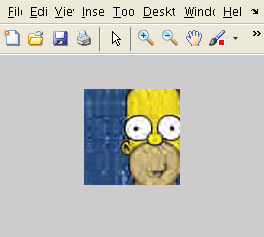
\includegraphics[height=6cm]{img/homero_10} 	
		\item \textbf{23\ Valores\ propios}\\
			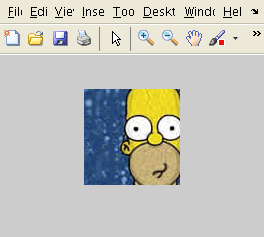
\includegraphics[height=6cm]{img/homero_23} 	
		\item \textbf{46\ Valores\ propios}\\
			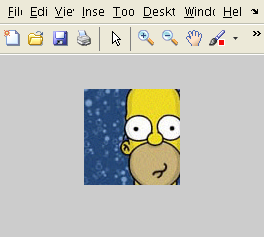
\includegraphics[height=6cm]{img/homero_46} 	
		\item \textbf{71\ Valores\ propios}\\
			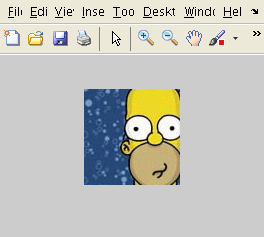
\includegraphics[height=6cm]{img/homero_71} 	
		\item \textbf{96\ Valores\ propios}\\
			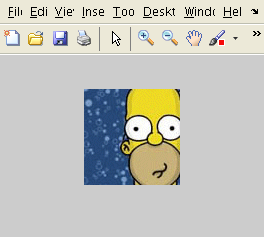
\includegraphics[height=6cm]{img/homero_96} 	
	\end{itemize}

Decidimos que con \emph{46 valores propios} ya se puede ver la imagen sin problema,
por lo tanto si pensamos que nuestra imagen es de \emph{96 valores propios} estamos realizando una reducción
de casi la mitad de valores propios, por lo cual podríamos pensar que podríamos reducir el tamaño del archivo
a la mitad, teniendo la misma información.
\newpage

\subsection{Utilizando otra factorizaci\'on, proponga otro m\'etodo para realizar el ejercicio, y concluya sobre sus resultados}

Encontramos que utilizando la factorización QR, logramos un procedimiento similar.

\begin{itemize}
	\item Obtenemos las matrices R,G y B de nuestra imagen.
	\item Por cada matriz aplicamos QR por separado.
	\item Descomponemos cada SVD, en una suma de matrices dependiendo de sus valores propios, es decir:\\
	$Q R = Q_1 R_1 + Q_2 R_2 + Q_3 R_3 + \ldots + Q_n R_n$
	\item Cada sub QR posee la columna n-ésima de $Q$ y la n-ésima fila de $R$
	\item Luego para poder ir probando la calidad de la imagen,
		vamos viendo la imagen para distintos $n$:\\
		$R = \sum_{k=1}^{n}Q_{R_{k}}R_{R_{k}}$\\
		$G = \sum_{k=1}^{n}Q_{G_{k}}R_{G_{k}}$\\
		$B = \sum_{k=1}^{n}Q_{B_{k}}R_{B_{k}}$
	\item Finalmente sobreponemos los nuevos R,G y B y mostramos la imagen para ver la calidad.
\end{itemize}

Nuevamente probaremos con distintos valores entre \emph{1 y 96}, que serian la cantidad de columnas de la matriz que ocuparemos.

	\begin{itemize}
		\item \textbf{10\ Columnas}\\
			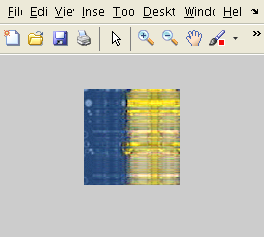
\includegraphics[height=6cm]{img/homeroQR_10} 	
		\item \textbf{23\ Columnas}\\
			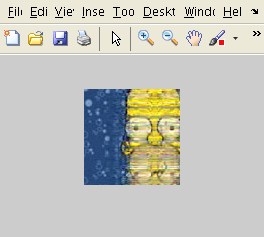
\includegraphics[height=6cm]{img/homeroQR_23} 	
		\item \textbf{46\ Columnas}\\
			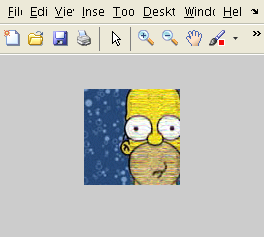
\includegraphics[height=6cm]{img/homeroQR_46} 	
		\item \textbf{71\ Columnas}\\
			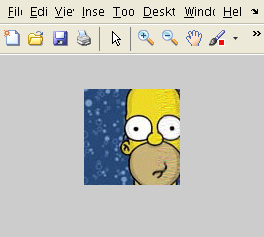
\includegraphics[height=6cm]{img/homeroQR_71} 	
		\item \textbf{96\ Columnas}\\
			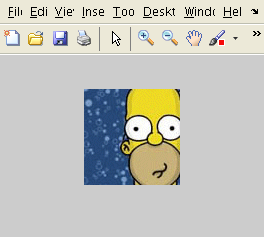
\includegraphics[height=6cm]{img/homeroQR_96} 	
	\end{itemize}

Claramente la imagen va a perdiendo calidad pero con franjas horizontales,
por lo cual es mucho mas complicado con este metodo y el 71 es mas parecido,
no como el caso anterior que con 46 valores propios funcionaba bien.

\newpage

\section{Segunda Parte}
\subsection{Sea $A$ $\in$ $\mathbb{R}^{nxn}$ aplique el algoritmo propuesto para $N$ $\in$
$[1,2,\cdots,N]$ hasta un $n$ razonable, ¿Cómo determino este $n$?}

Primero describiremos el método. Se comienza con una matriz invertible $A$, $n x n$. Se calcula la
factorización $QR$ de $A$ = $QR$, y a continuación se forma la matriz $A_1 = RQ$. Observaremos que $A$ y
$A_1$ son semejantes, porque:
$$
	Q^{-1} AQ = Q^{-1} (QR) Q = RQ = A_1
$$
Por tanto, tienen los mismos valores propios. Continuamos con la factorización $QR$, $R_1Q_1$ de $A_1$, y se forma
la matriz $A_2 = Q_1 R_1$ que tiene los mismos valores propios que $A$. Iteramos para obtener una sucesión de
matrices
$$
	A, A_1, A_2, A_3, \cdots
$$
Resultando que si $A$ tiene $n$ valores propios de distintas magnitudes, entonces basta iterar hasta tal
$n$ para obtener una matriz triangular superior $\hat{R}$ semejante a $A$. De todas formas, el algoritmo
no posee un término formal para sus iteraciones. Mientras más se itere, más uno se acercará a la matriz.

\subsection{Examine los valores de $diag(A_N)$, ¿a que corresponden?}

Resulta que si $A$ tiene $n$ valores propios de distintas magnitudes, entonces esta sucesión tiende a una
matriz triangulas superior $\hat{R}$ semejante a $A$.
Por consiguiente, los elementos diagonales de $\hat{R}$ son todos los valores propios de $A$.
El algoritmo y teorema siguiente, cuya demostración omitiremos, es el núcleo del método $QR$ que acabamos
de describir.

\subsection{El algoritmo planteado es conocido, investigue brevemente al respecto.}
\textbf{Método $QR$ para valores propios}
 
La descomposición $QR$ puede usarse para aproximar los valores propios de una matriz cuadrada. Al algoritmo
resultante se le llama método $QR$, y constituye una herramienta importante para aproximaciones numéricas
de los valores propios. Comparado con los demás, el método $QR$ determina todos los valores propios de una
matriz. También se usa para resolver sistemas lineales. Además, en la ortonormalización se emplean sus
variantes para reemplazar el proceso de Gram-Schmidt, que es inestable.

Resulta que si $A$ tiene $n$ valores propios de distintas magnitudes, entonces esta sucesión tiende a una
matriz triangulas superior $\hat{R}$ semejante a $A$.
Por consiguiente, los elementos diagonales de $\hat{R}$ son todos los valores propios de $A$.\\

\textbf{El método $QR$:}
\begin{description}
	\item[Datos:] Para una matriz $A$ invertible $n x n$, cuyos valores propios son
	$\lambda_1$,$\cdots$,$\lambda_n$, tal que:
$$
		\lvert\lambda_1\rvert>\lvert\lambda_2\rvert>...>\lvert\lambda_n\rvert
$$
	\begin{enumerate}	
		\item Igualar $A_0$ = $A$.
		\item Para $i = 1,2,\cdots, k-1$:
		\begin{enumerate}
			\item Determinar la descomposición $QR$ de $A_i$, por ejemplo $A_i = Q_i R_i$.
			\item Igualar $A_{i+1} = R_iQ_i$.
		\end{enumerate}
	\end{enumerate}
	\item[Resultados:] $A_k$, que se aproxima a una matriz triangular $\hat{R}$ cuyos elementos diagonales
	son todos los valores propios de $A$.
\end{description}

Una nota sobre el método QR, es que en la descomposición QR, la matriz R no es exactamente triangular después del cálculo numérico. Los elementos que deberían ser cero con frecuencia son números muy pequeños. En la práctica, se pasa directamente a las aproximaciones.

\newpage

\end{document}
